%%%%%%%%%%%%%%%%%%%%%%%%%%%%%%%%%%%%

\begin{frame}
Section 1.2: Data Basics
\end{frame}

%%%%%%%%%%%%%%%%%%%%%%%%%%%%%%%%%%%%

%\subsection{Definitions}

\begin{frame}
\frametitle{Some definitions}

\begin{itemize}
\item {\bf Data:} \pause Observations, measurements, and information that is analyzed. \pause
\item {\bf Summary statistic:} \pause A single number summarizing a large amount of data. \pause
\item {\bf Data matrix:} \pause A collection of data with each row a case and each column a variable. \pause
\item {\bf Case:} \pause An observational unit. \pause
\item {\bf Variable:} \pause A characteristic (usually one of many) that is measured from each case.
%\item For example, if you are testing the effects of a drug, the cases are the patients and the variables would be things like gender, height, weight, preconditions, blood pressure, death rate, happiness, amount of sleep, weight change, etc...
\end{itemize}

\end{frame}




%\subsection{Observations and variables}

%\begin{frame}
%\frametitle{Data matrix}

%Data collected on students in a statistics class on a variety of variables:

%\begin{center}
%\begin{tabular}{l cccc l}
%		& \hl{variable} \\
%		& \hl{$\downarrow$}	 \\
%\cline{1-5}
%Stu.	&	\var{gender}	&	\var{intro\_extra} & $\cdots$ & \var{dread} \\
%\cline{1-5}
%1 & male & extravert  & $\cdots$ & 3 \\ 
%  2 & female & extravert & $\cdots$ & 2 \\ 
%  3 & female & introvert  & $\cdots$ & 4 & \hl{$\leftarrow$ case}  \\ 
%  4 & female & extravert  & $\cdots$ & 2 &  \\
%$\vdots$	&	$\vdots$	  &	$\vdots$  &	$\vdots$ &	$\vdots$ \\
%86	& male & extravert & $\cdots$& 3 \\
%\cline{1-5}
%\end{tabular}
%\end{center}

%\end{frame}

%%%%%%%%%%%%%%%%%%%%%%%%%%%%%%%%%%%%

%\subsection{Types of variables}

\begin{frame}
\frametitle{Types of variables}

\begin{center}
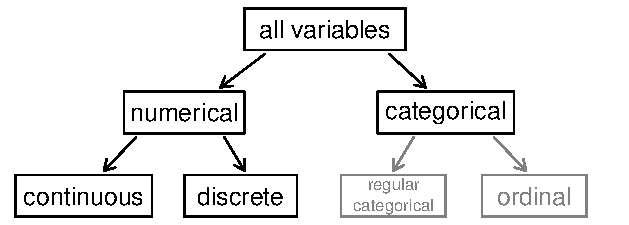
\includegraphics[width=0.8\textwidth]{1-2_data_basics/figures/variables/variables}
\end{center}

\begin{itemize}
\item Numerical variables take values that can be added, subtracted, and averaged in a sensible way.
\item Discrete numerical variables take on values with jumps e.g. counts, ``how many''.
\item Continuous numerical variables take on values without jumps e.g. weights, heights, ''how much''.
\end{itemize}

\end{frame}


\begin{frame}
\frametitle{Types of variables 2}

\begin{center}
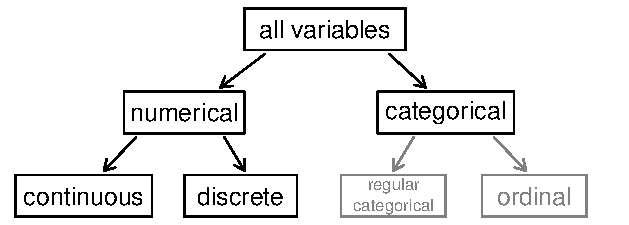
\includegraphics[width=0.8\textwidth]{1-2_data_basics/figures/variables/variables}
\end{center}
\begin{itemize}
\item Categorical variables do not take values that can be added, subtracted, and averaged in a sensible way.
\end{itemize}
\end{frame}

%%%%%%%%%%%%%%%%%%%%%%%%%%%%%%%%%%%

%\subsection{Quiz}

\begin{frame}[fragile]
\frametitle{Practice}
{\scriptsize
\begin{verbatim}
> mtcars
                     mpg cyl  disp  hp drat    wt  qsec vs am gear carb
Mazda RX4           21.0   6 160.0 110 3.90 2.620 16.46  0  1    4    4
Mazda RX4 Wag       21.0   6 160.0 110 3.90 2.875 17.02  0  1    4    4
Datsun 710          22.8   4 108.0  93 3.85 2.320 18.61  1  1    4    1
Hornet 4 Drive      21.4   6 258.0 110 3.08 3.215 19.44  1  0    3    1
Hornet Sportabout   18.7   8 360.0 175 3.15 3.440 17.02  0  0    3    2
Valiant             18.1   6 225.0 105 2.76 3.460 20.22  1  0    3    1
Duster 360          14.3   8 360.0 245 3.21 3.570 15.84  0  0    3    4
Merc 240D           24.4   4 146.7  62 3.69 3.190 20.00  1  0    4    2
Merc 230            22.8   4 140.8  95 3.92 3.150 22.90  1  0    4    2
Merc 280            19.2   6 167.6 123 3.92 3.440 18.30  1  0    4    4
Merc 280C           17.8   6 167.6 123 3.92 3.440 18.90  1  0    4    4
Merc 450SE          16.4   8 275.8 180 3.07 4.070 17.40  0  0    3    3
Merc 450SL          17.3   8 275.8 180 3.07 3.730 17.60  0  0    3    3
Merc 450SLC         15.2   8 275.8 180 3.07 3.780 18.00  0  0    3    3
Cadillac Fleetwood  10.4   8 472.0 205 2.93 5.250 17.98  0  0    3    4
\end{verbatim}}
Cases? Variables? Types of Variables?

\end{frame}


\begin{frame}[fragile]
\frametitle{Variable descriptions}
\begin{verbatim}
mtcars
A data frame with 32 observations on 11 variables.

[, 1]  mpg   Miles/(US) gallon                        
[, 2]  cyl   Number of cylinders                      
[, 3]  disp  Displacement (cu.in.)                    
[, 4]  hp    Gross horsepower                         
[, 5]  drat  Rear axle ratio                          
[, 6]  wt    Weight (1000 lbs)                        
[, 7]  qsec  1/4 mile time                            
[, 8]  vs    V/S                                      
[, 9]  am    Transmission (0 = automatic, 1 = manual) 
[,10]  gear  Number of forward gears                  
[,11]  carb  Number of carburetors                         
\end{verbatim}
\end{frame}


\begin{frame}
\frametitle{Types of variables (cont.)}

\begin{center}
{\footnotesize
\begin{tabular}{c ccc cc}
  \hline
 & \var{gender} & \var{sleep (hr)} & \var{bedtime} & \var{countries} & \var{dread} \\
  \hline
1 & male & 5 & 12-2 & 13 & 3 \\ 
  2 & female & 7 & 10-12 & 7 & 2 \\ 
  3 & female & 5.5 & 12-2 & 1 & 4 \\ 
  4 & female & 7 & 12-2 &  & 2 \\ 
  5 & female & 3 & 12-2 & 1 & 3 \\ 
  6 & female & 3 & 12-2 & 9 & 4 \\ 
  \hline
\end{tabular}
}
\end{center}

\begin{itemize}
\item \var{gender}: \pause \soln{\only<2->{categorical}} \pause
\item \var{sleep}: \pause \soln{\only<4->{numerical, continuous}} \pause
\item \var{bedtime}: \pause \soln{\only<6->{categorical, ordinal}} \pause
\item \var{countries}: \pause \soln{\only<8->{numerical, discrete}} \pause
\item \var{dread}: \pause \soln{\only<10->{categorical, ordinal - could also be used as numerical}}
\end{itemize}

\end{frame}

%%%%%%%%%%%%%%%%%%%%%%%%%%%%%%%%%%%

\begin{frame}
\frametitle{Practice}

\pq{What type of variable is a telephone area code?}

\begin{enumerate}[(a)]
\item numerical, continuous
\item numerical, discrete
\solnMult{categorical}
\item categorical, ordinal
\end{enumerate}

\end{frame}



%\section{Relationships among variables}

\begin{frame}
\frametitle{Positive association}

\begin{center}
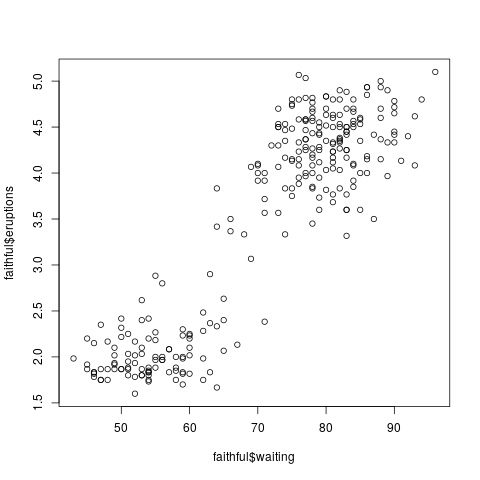
\includegraphics[width=0.6\textwidth]{1-2_data_basics/figures/faithful/faithful}
\end{center}

\small
The eruption time (min) vs wait time (min) for 272 cases of Old Faithful.

\end{frame}

\begin{frame}
\frametitle{Negative association}

\begin{center}
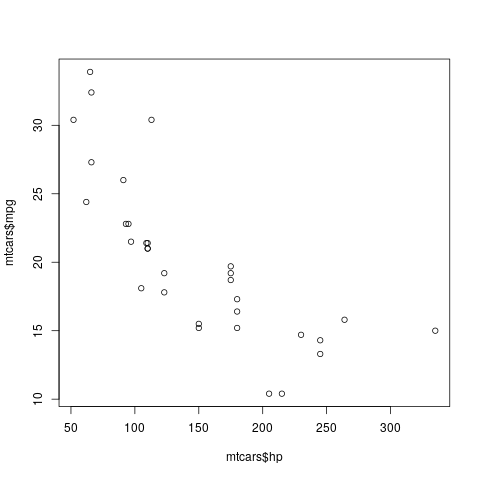
\includegraphics[width=0.6\textwidth]{1-2_data_basics/figures/cars/cars}
\end{center}

\small
The mpg vs. HP for 32 cars.

\end{frame}


\begin{frame}
\frametitle{Independent variables}

\begin{center}
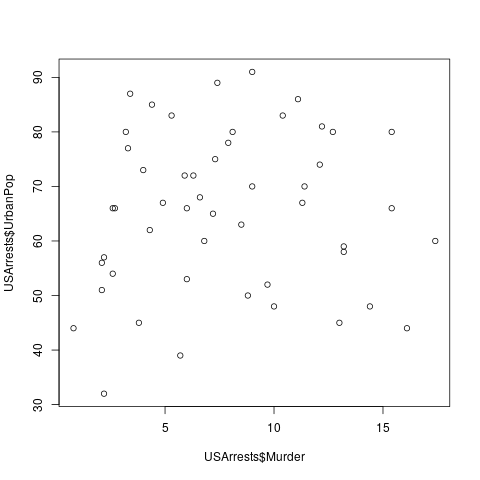
\includegraphics[width=0.6\textwidth]{1-2_data_basics/figures/urbmur/urbmur}
\end{center}

\small
From 1973, murder rate vs urban population proportion (50 states).

\end{frame}


%%%%%%%%%%%%%%%%%%%%%%%%%%%%%%%%%%%

%\subsection{Relationships among variables}

%%%%%%%%%%%%%%%%%%%%%%%%%%%%%%%%%%%

\begin{frame}
\frametitle{Relationships among variables}

\dq{Does there appear to be a relationship between GPA and number of hours students study per week?}

\begin{center}
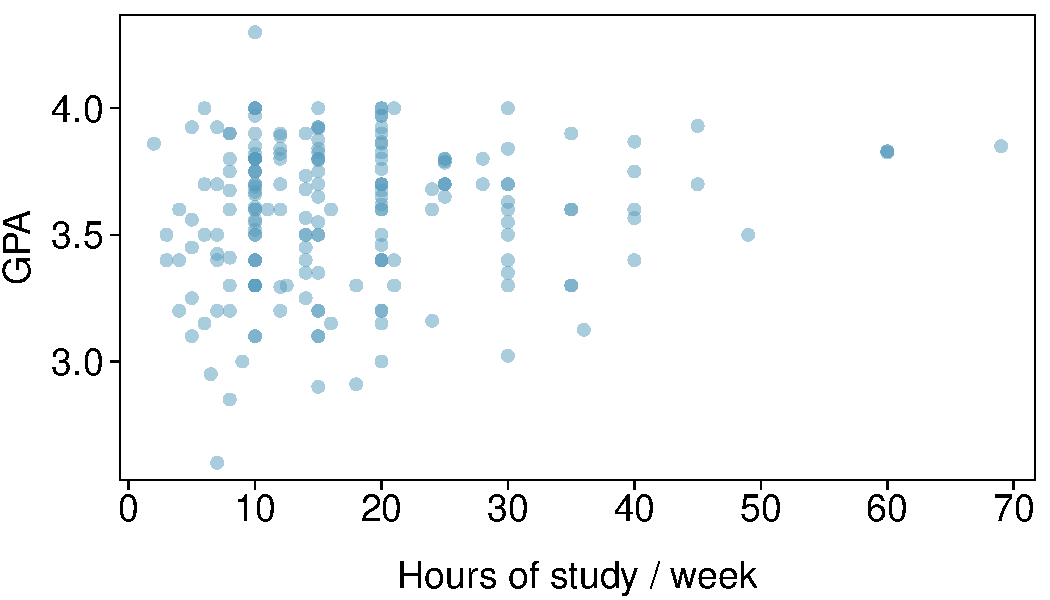
\includegraphics[width=0.7\textwidth]{1-2_data_basics/figures/gpa_study_hours/gpa_study_hours}
\end{center}

\pause

\dq{Can you spot anything unusual about any of the data points?}

\soln{\pause{There is one student with GPA $>$ 4.0, this is likely a data error.}}

\end{frame}

%%%%%%%%%%%%%%%%%%%%%%%%%%%%%%%%%%%

%\subsection{Associated and independent variables}

%%%%%%%%%%%%%%%%%%%%%%%%%%%%%%%%%%%

\begin{frame}
\frametitle{Practice}

\twocol{0.5}{0.5}
{
\pq{Based on the scatterplot on the right, which of the following statements is correct about the head and skull lengths of possums?}
}
{
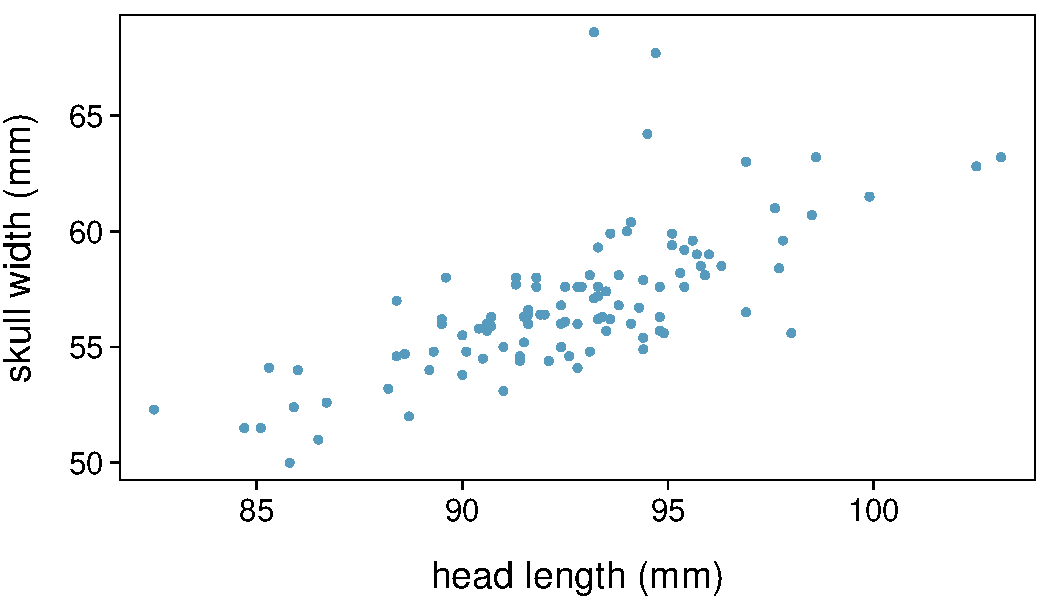
\includegraphics[width=\textwidth]{1-2_data_basics/figures/possum_head_skull/possum_head_skull}
}

\begin{enumerate}[(a)]
\item There is no relationship between head length and skull width, i.e. the variables are independent.
\solnMult{Head length and skull width are positively associated.}
\item Skull width and head length are negatively associated.
\item A longer head causes the skull to be wider.
\item A wider skull causes the head to be longer.
\end{enumerate}

\end{frame}

%%%%%%%%%%%%%%%%%%%%%%%%%%%%%%%%%%%

\begin{frame}
\frametitle{Associated vs. independent}

\begin{itemize}

\item When two variables show some connection with one another, they are called \hl{associated} variables.
\begin{itemize}
\item Associated variables can also be called \hl{dependent} variables and vice-versa.
\end{itemize}

\item If two variables are not associated, i.e. there is no evident connection between the two, then they are said to be \hl{independent}.

\end{itemize}

\end{frame}

%%%%%%%%%%%%%%%%%%%%%%%%%%%%%%%%%%%%


\begin{frame}
\frametitle{Class survey}
What would be some interesting questions we could ask everyone in the room?

For each question, what type of variable would be recorded?

Would the survey be anonymous?

Which variables would you expect to be associated? independent?

\end{frame}


